\documentclass[a4paper,12pt]{article}

\usepackage{amsmath}
\usepackage{subcaption}
\usepackage{pgfplots}
\usepackage{tikz}
\usepackage{xspace}
\usepackage{listings}

\pgfplotsset{
  label style={font=\scriptsize},
  tick label style={font=\scriptsize},
  legend style={font=\scriptsize},
}

\makeatletter
\lstdefinestyle{mystyle}{
  basicstyle=%
    \ttfamily
    %\color{blue}%
    \lst@ifdisplaystyle\scriptsize\fi
}
\makeatother
\lstset{style=mystyle}

\newcommand*{\hard}{\lstinline!hard!\@\xspace}
\newcommand*{\moderate}{\lstinline!moderate!\@\xspace}
\newcommand*{\easy}{\lstinline!easy!\@\xspace}

\newcommand*{\PPCA}{\lstinline!PPCA!\@\xspace}
\newcommand*{\VAE}{\lstinline!VAE!\@\xspace}
\newcommand*{\DVAE}{\lstinline!DVAE!\@\xspace}
\newcommand*{\VAEs}{\lstinline!VAEs!\@\xspace}
\newcommand*{\DVAEs}{\lstinline!DVAEs!\@\xspace}
\newcommand*{\ML}{\lstinline!ML!\@\xspace}
\newcommand*{\DL}{\lstinline!DL!\@\xspace}
\newcommand*{\AML}{\lstinline!AML!\@\xspace}
\newcommand*{\EVAE}{\lstinline!EVAE!\@\xspace}
\newcommand*{\EVAEs}{\lstinline!EVAEs!\@\xspace}

\def\NLL{\text{NLL}\xspace}
\def\Abs{\text{Abs}\xspace}
\DeclareRobustCommand{\AbsThr}{%
    \ifmmode
        \text{Abs}_{\text{thresh}}
    \else
        $\text{Abs}_{\text{thresh}}$
    \fi
}

% https://tex.stackexchange.com/questions/13627/pgfplots-multiple-shifted-stacked-plots-in-one-diagram
\makeatletter
\newcommand\resettenstackedplots{
\makeatletter
\pgfplots@stacked@isfirstplottrue
\makeatother
\addplot [forget plot,draw=none] coordinates{
  (1,0) (2,0) (3,0) (4, 0) (5, 0)
  (6,0) (7,0) (8,0) (9, 0) (10, 0)
};
}
\makeatother
\makeatletter
\newcommand\resetelevenstackedplots{
\makeatletter
\pgfplots@stacked@isfirstplottrue
\makeatother
\addplot [forget plot,draw=none] coordinates{
  (1,0) (2,0) (3,0) (4, 0) (5, 0)
  (6,0) (7,0) (8,0) (9, 0) (10, 0)
  (11, 0)
};
}
\makeatother
\makeatletter
\newcommand\resettwelvestackedplots{
\makeatletter
\pgfplots@stacked@isfirstplottrue
\makeatother
\addplot [forget plot,draw=none] coordinates{
  (1,0) (2,0) (3,0) (4, 0) (5, 0)
  (6,0) (7,0) (8,0) (9, 0) (10, 0)
  (11, 0) (12, 0)
};
}
\makeatother

\begin{document}
  
\begin{figure}
  \centering
  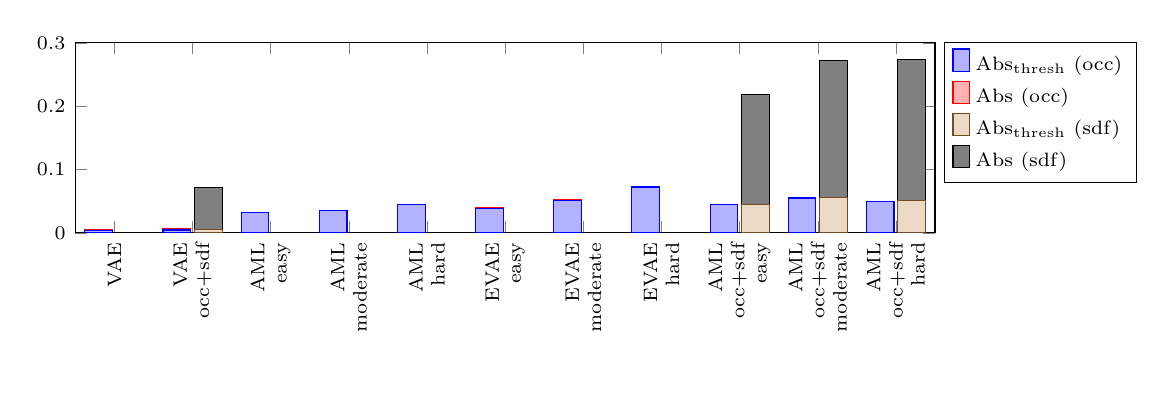
\begin{tikzpicture}
    \begin{axis}[
        ybar stacked,
        % https://tex.stackexchange.com/questions/119887/remove-the-scientific-notation-which-is-unreasonable
        yticklabel style={
          /pgf/number format/fixed,
          /pgf/number format/precision=5
        },
        scaled y ticks=false,
        %enlargelimits=0.15,
        legend style={
          at={(1.01,1)},
          anchor=north west,
        },
        % https://tex.stackexchange.com/questions/48620/pgfplots-alignment-and-size-of-math-in-legend
        legend cell align=left,
        xtick={
          1, 2,
          3, 4, 5,
          6, 7, 8,
          9, 10, 11
        },
        xticklabels={
          \VAE, \VAE occ+sdf,
          \AML\\\easy, \AML\\\moderate, \AML \\\hard,
          \EVAE\\\easy, \EVAE\\\moderate, \EVAE\\\hard,
          \AML occ+sdf\\\easy, \AML occ+sdf\\\moderate, \AML occ+sdf\\\hard
        },
        x tick label style={text width=1.5cm,align=right},
        ymin=0,
        width=12.5cm,
        height=4cm,
        % https://tex.stackexchange.com/questions/271027/pgfplots-how-to-rotate-extra-x-tick-labels
        x tick label style={
          rotate=90,
          anchor=east,
        },
        enlarge x limits=0.05,
        % https://tex.stackexchange.com/questions/47882/formatting-a-pgfplot-graph-thicker-bars-and-total-width
        %bar width=8,
      ]
        
      % AbsThr
      \addplot +[bar shift=-.2cm] coordinates {
        (1, 0.00384198)
        (2, 0.00453785)
        (3, 0.03217211)
        (4, 0.03567748)
        (5, 0.04434539)
        %
        (6, 0.03876815)
        (7, 0.05154616)
        (8, 0.07254225)
        %
        (9, 0.04437874)
        (10, 0.05507257)
        (11, 0.0500495)
      };
      \addlegendentry{\AbsThr (occ)}
      % Abs
      \addplot +[bar shift=-.2cm] coordinates {
        (1, 0.00155) % 0.00539829)
        (2, 0.001953) % 0.00649281)
        (3, 0.000155) % 0.03232507)
        (4, 0.000218) % 0.03588854)
        (5, 0.000445) % 0.04479165)
        %
        (6, 0.00072) % 0.03942102)
        (7, 0.0003) % 0.05189751)
        (8, 0.00031) % 0.07285957)
        %
        (9, 0.0002) % 0.04457945)
        (10, 0.00016) % 0.05523896)
        (11, 0.00019) % 0.05023721)
      };
      \addlegendentry{\Abs (occ)}
      
      % --
      \resetelevenstackedplots
      
      % AbsThr
      \addplot +[bar shift=+.2cm] coordinates {
        (1, 0)
        (2, 0.00534606)
        (3, 0)
        (4, 0)
        (5, 0)
        %
        (6, 0)
        (7, 0)
        (8, 0)
        %
        (9, 0.04459624)
        (10, 0.05582422)
        (11, 0.05130592)
      };
      \addlegendentry{\AbsThr (sdf)}
      % Abs
      \addplot +[bar shift=+.2cm] coordinates {
        (1, 0)
        (2, 0.06582) % 0.07112682)
        (3, 0)
        (4, 0)
        (5, 0)
        %
        (6, 0)
        (7, 0)
        (8, 0)
        %
        (9, 0.17411) % 0.21871304)
        (10, 0.21636) % 0.27216289)
        (11, 0.2225) % 0.27388566)
      };
      \addlegendentry{\Abs (sdf)}
    \end{axis}
  \end{tikzpicture}
\end{figure}

\begin{figure}
  \centering
  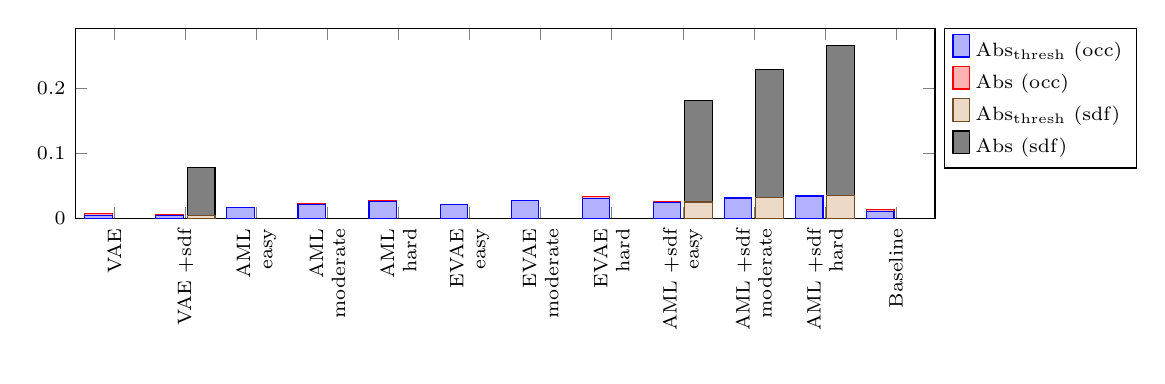
\begin{tikzpicture}
    \begin{axis}[
        ybar stacked,
        % https://tex.stackexchange.com/questions/119887/remove-the-scientific-notation-which-is-unreasonable
        yticklabel style={
          /pgf/number format/fixed,
          /pgf/number format/precision=5
        },
        scaled y ticks=false,
        %enlargelimits=0.15,
        legend style={
          at={(1.01,1)},
          anchor=north west,
        },
        % https://tex.stackexchange.com/questions/48620/pgfplots-alignment-and-size-of-math-in-legend
        legend cell align=left,
        xtick={
          1, 2,
          3, 4, 5,
          6, 7, 8,
          9, 10, 11,
          12
        },
        xticklabels={
          \VAE, \VAE +sdf,
          \AML\\\easy, \AML\\\moderate, \AML\\\hard,
          \EVAE\\\easy, \EVAE\\\moderate, \EVAE\\\hard,
          \AML +sdf\\\easy, \AML +sdf\\\moderate, \AML +sdf\\\hard,
          Baseline
        },
        x tick label style={text width=1.5cm,align=right},
        ymin=0,
        width=12.5cm,
        height=4cm,
        enlarge x limits=0.05,
        % https://tex.stackexchange.com/questions/271027/pgfplots-how-to-rotate-extra-x-tick-labels
        x tick label style={
          rotate=90,
          anchor=east,
        },
        %bar width=8,
      ]
      
      % AbsThr
      \addplot +[bar shift=-.2cm] coordinates {
        (1, 0.00505722)
        (2, 0.00475067)
        (3, 0.01667228)
        (4, 0.0215971)
        (5, 0.02619364)
        %
        (6, 0.02136223)
        (7, 0.02775098)
        (8, 0.03063716)
        %
        (9, 0.02538469)
        (10, 0.03168048)
        (11, 0.03483872)
        (12, 0.010504529630079)
      };
      \addlegendentry{\AbsThr (occ)}
      % Abs
      \addplot +[bar shift=-.2cm] coordinates {
        (1, 0.002275) % 0.00733222)
        (2, 0.00203) % 0.00678092)
        (3, 0.00101) % 0.01768816)
        (4, 0.00088) % 0.02247298)
        (5, 0.00099) % 0.02718333)
        %
        (6, 0.00083) % 0.02219768)
        (7, 0.00063) % 0.02838561)
        (8, 0.0031) % 0.03373657)
        %
        (9, 0.00051) % 0.02589711)
        (10, 0.00041) % 0.0320905)
        (11, 0.00019) % 0.0350219)
        (12, 0.003366) % 0.013873896760899)
      };
      \addlegendentry{\Abs (occ)}
      
      % -- 
      \resettwelvestackedplots
      
      % AbsThr
      \addplot +[bar shift=+.2cm] coordinates {
        (1, 0)
        (2, 0.00530342)
        (3, 0)
        (4, 0)
        (5, 0)
        %
        (6, 0)
        (7, 0)
        (8, 0)
        %
        (9, 0.02553955)
        (10, 0.03210551)
        (11, 0.03564795)
        (12, 0)
      };
      \addlegendentry{\AbsThr (sdf)}
      % Abs
      \addplot +[bar shift=+.2cm] coordinates {
        (1, 0)
        (2, 0.0733) % 0.07860103)
        (3, 0)
        (4, 0)
        (5, 0)
        %
        (6, 0)
        (7, 0)
        (8, 0)
        %
        (9, 0.15607) % 0.18164451)
        (10, 0.1978) % 0.2299151)
        (11, 0.2304) % 0.26641559)
        (12, 0)
      };
      \addlegendentry{\Abs (sdf)}
    \end{axis}
  \end{tikzpicture}
\end{figure}

\end{document}